


\tikzset{every picture/.style={line width=0.75pt}} %set default line width to 0.75pt        

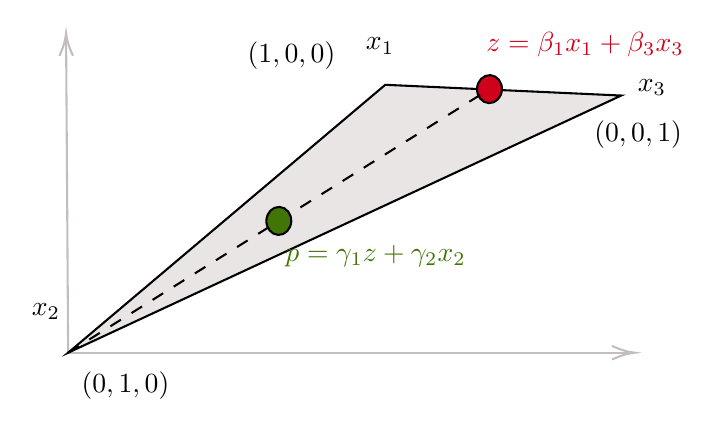
\begin{tikzpicture}[x=0.75pt,y=0.75pt,yscale=-1,xscale=1]
	%uncomment if require: \path (0,300); %set diagram left start at 0, and has height of 300
	
	%Straight Lines [id:da574149972137515] 
	\draw [color={rgb, 255:red, 195; green, 190; blue, 190 }  ,draw opacity=1 ]   (33,258.5) -- (304,258.5) ;
	\draw [shift={(306,258.5)}, rotate = 180] [color={rgb, 255:red, 195; green, 190; blue, 190 }  ,draw opacity=1 ][line width=0.75]    (10.93,-3.29) .. controls (6.95,-1.4) and (3.31,-0.3) .. (0,0) .. controls (3.31,0.3) and (6.95,1.4) .. (10.93,3.29)   ;
	%Straight Lines [id:da6051947502547008] 
	\draw [color={rgb, 255:red, 195; green, 190; blue, 190 }  ,draw opacity=1 ]   (33,258.5) -- (32.01,106.5) ;
	\draw [shift={(32,104.5)}, rotate = 89.63] [color={rgb, 255:red, 195; green, 190; blue, 190 }  ,draw opacity=1 ][line width=0.75]    (10.93,-3.29) .. controls (6.95,-1.4) and (3.31,-0.3) .. (0,0) .. controls (3.31,0.3) and (6.95,1.4) .. (10.93,3.29)   ;
	%Shape: Right Triangle [id:dp9642640346709239] 
	\draw  [fill={rgb, 255:red, 234; green, 229; blue, 229 }  ,fill opacity=1 ] (299.48,134.6) -- (33,258.5) -- (185.8,129.42) -- cycle ;
	%Shape: Ellipse [id:dp24503782326315404] 
	\draw  [fill={rgb, 255:red, 208; green, 2; blue, 27 }  ,fill opacity=1 ] (230.01,131.2) .. controls (230.19,127.48) and (233.02,124.6) .. (236.33,124.76) .. controls (239.64,124.92) and (242.18,128.07) .. (241.99,131.8) .. controls (241.81,135.52) and (238.98,138.4) .. (235.67,138.24) .. controls (232.36,138.08) and (229.82,134.93) .. (230.01,131.2) -- cycle ;
	%Straight Lines [id:da21833955225597546] 
	\draw  [dash pattern={on 4.5pt off 4.5pt}]  (33,258.5) -- (236,131.5) ;
	%Shape: Ellipse [id:dp28236760411930684] 
	\draw  [fill={rgb, 255:red, 65; green, 117; blue, 5 }  ,fill opacity=1 ] (128.51,194.7) .. controls (128.69,190.98) and (131.52,188.1) .. (134.83,188.26) .. controls (138.14,188.42) and (140.68,191.57) .. (140.49,195.3) .. controls (140.31,199.02) and (137.48,201.9) .. (134.17,201.74) .. controls (130.86,201.58) and (128.32,198.43) .. (128.51,194.7) -- cycle ;
	
	% Text Node
	\draw (118,107.4) node [anchor=north west][inner sep=0.75pt]    {$( 1,0,0)$};
	% Text Node
	\draw (285,145.4) node [anchor=north west][inner sep=0.75pt]    {$( 0,0,1)$};
	% Text Node
	\draw (38,266.4) node [anchor=north west][inner sep=0.75pt]    {$( 0,1,0)$};
	% Text Node
	\draw (175,105.4) node [anchor=north west][inner sep=0.75pt]    {$x_{1}$};
	% Text Node
	\draw (306,125.4) node [anchor=north west][inner sep=0.75pt]    {$x_{3}$};
	% Text Node
	\draw (14,233.4) node [anchor=north west][inner sep=0.75pt]    {$x_{2}$};
	% Text Node
	\draw (233,102.4) node [anchor=north west][inner sep=0.75pt]  [color={rgb, 255:red, 208; green, 2; blue, 27 }  ,opacity=1 ]  {$z=\beta _{1} x_{1} +\beta _{3} x_{3} \ $};
	% Text Node
	\draw (136.17,205.14) node [anchor=north west][inner sep=0.75pt]  [color={rgb, 255:red, 65; green, 117; blue, 5 }  ,opacity=1 ]  {$p=\gamma _{1} z+\gamma _{2} x_{2}$};
	
	
\end{tikzpicture}
